 \documentclass[a4paper,12pt]{report}

\usepackage[utf8]{inputenc}
\usepackage[T1]{fontenc}
\usepackage{array}
\usepackage{amsmath}
\usepackage[english]{babel}
\usepackage{graphicx}
\usepackage[a4paper]{geometry}
\usepackage[colorlinks=true,urlcolor=blue,linkcolor=blue]{hyperref}
\usepackage{url}
\usepackage[nottoc,numbib]{tocbibind}
\usepackage{color}
\usepackage{epstopdf}
\usepackage{xcolor}
\usepackage[backend=biber,style=phys]{biblatex}
\usepackage{lipsum}
\usepackage[capbesideposition={right,center}]{floatrow}
\usepackage[ampersand]{easylist}

\addbibresource{../Bibliography.bib}
\makeatletter
	\renewcommand{\thechapter}{\Roman{chapter}}
\makeatother

\newcolumntype{M}[1]{>{\centering\arraybackslash}m{#1}}

\floatsetup[table]{style=plaintop}

\begin{document}

\chapter{Growth and first characterization of Cr-doped CdTe quantum dots\label{Growth}}

%	The growth took place at Tsukuba University, in the team of Pr. Shinji Kuroda. The samples were grown with Molecular Beam Epitaxy (MBE) and Atomic Layer Epitaxy (ALE, for the QD layer), via individual Cd, Te, Zn, Mg and Cr cells. MBE and ALE are two complementary techniques for the growth of semiconductor device.
	During this thesis, we studied two types of magnetic QDs: self assembled QDs and strain free QDs. The formers are formed by the partial relaxation of the strain of a CdTe layer on a ZnTe substrate (Stranski-Krastanov dots). Strain free dots are formed by thickness variation of a CdTe /CdMgTe thin quantum well (QW) on a CdTe substrate. The growth of Cr doped samples were done in Pr. Shinji Kuroda laboratory, in the University of Tsukuba. The Mn-doped samples were grown at Grenoble, in the CEA-CNRS joined team NPSC, by Dr. Herv\'e Boukari.
	
	We will focus in this chapter on the growth done at Tsukuba by Molecular Beam Epitaxy (MBE). We begin with some general explanation on the MBE process and the different tools that are used in it. We then go to the growth of the self-assembled Cr-doped QDs, explaining the preparation of the substrate, the growth, and discussing the first characterization of the samples. In the last section, we present two other kinds of samples we grew: samples with the possibility of applying an electric field on them, and the strain free dots. For each of them, we explain the growth process and present basic characterization. 
	
	\section{The Molecular Beam Expitaxy}	
	
	The samples we used are grown using epitaxy. It consists on depositing atoms or molecules on the surface of the sample. Each elements are deposited on top of each other, and the lattice parameter of the substrate in the plane is kept as long as no defect appears in the material. The elements condensate on the surface, where they can diffuse before getting adsorbed, or re-evaporate in the gas. The substrate temperature is tuned in order to maximise the mobility of the elements, to get a flat surface, while minimizing the re-evaporation. To achieve such a growth, we used a process called Molecular Beam Epitaxy (MBE), in which flux of elements are evaporated toward the sample, where each atom or molecule is deposited and crystallize. This is done using cells of elements heated to control their evaporation or until they reach sublimation.

	The MBE process was first devised at the end of the 1960s~\cite{FirstMBE}. This method offers a good control on the growth, which makes it useful for the development of nanostructures. Depositing the materials layer by layer gives the possibility to grow really thin structure, and the transition between two materials can be made really abrupt, with the possibility to go from one material to another over a single monolayer (ML).
	
	\begin{figure}[h!]
	\begin{center}
		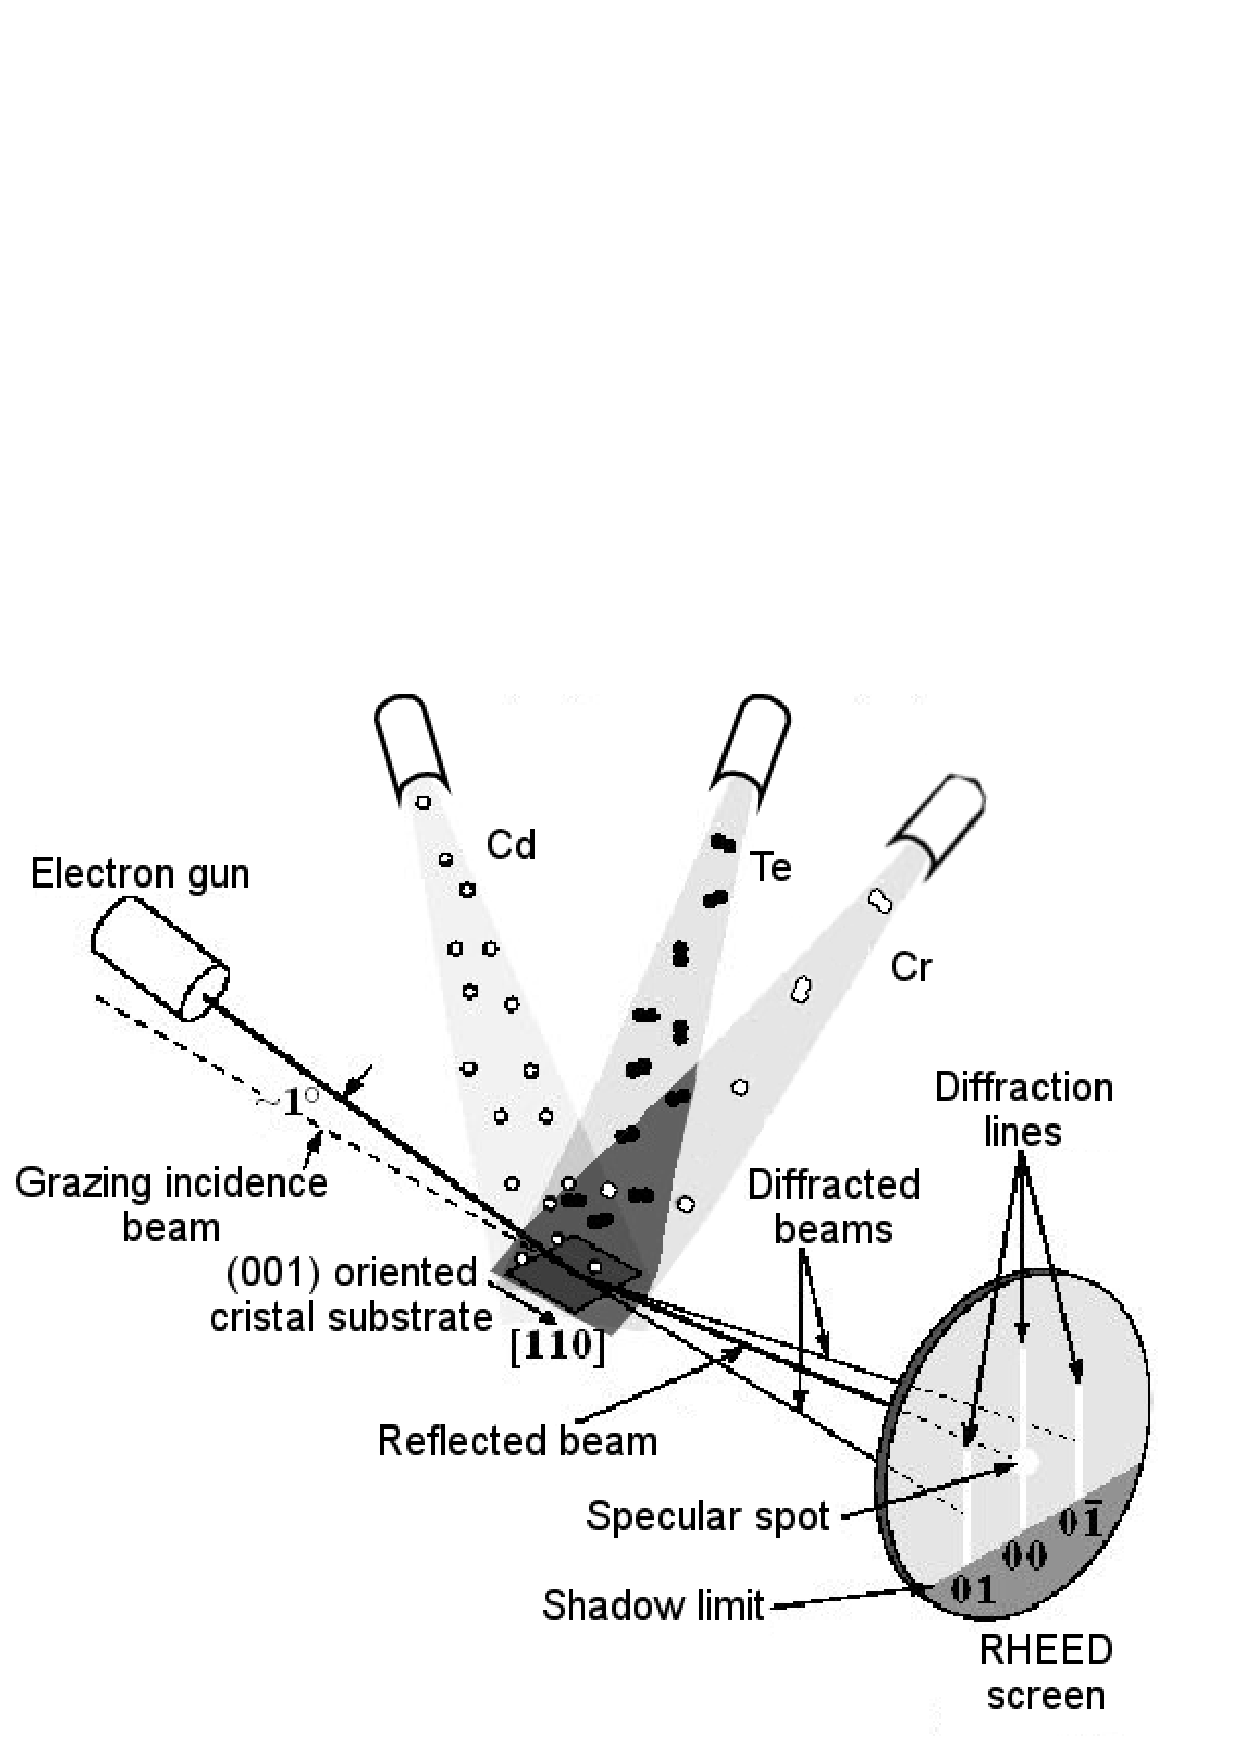
\includegraphics[width=10cm]{Pictures/MBE.png}
	\end{center}
	\caption{Schema of MBE cells and substrate during a growth. An electron gun is attached to the chamber in order to probe the surface of the sample.}
	\label{MBEScheme}
	\end{figure}
	
	 The elements are kept in Knudsen cells, which consist of a crucible of high-melting-point material wrapped in Tungsten filament acting as heater. A shutter is put in front of them to stop the element flux. During the growth, the shutter is opened to let the element travel to the substrate. The growth by MBE is a slow process: it can take more than a hour to get a layer 1 $\mu$m thick. In order to avoid contamination, Ultra High Vacuum, in the order of $10^{-8}$ Pa, is needed. Under this condition, the mean free path of the gas is long compared to distance to the sample (km for the mean free path of gas, when the distance between the substrate and the cell is of the order of 50 cm). This process is illustrated in Fig.~\ref{MBEScheme}. Reaching the surface, the atoms diffuse before stopping, either having dissipated their kinetic energy through interaction with the surface, or (more commonly) being kept by steps created by previously deposited atoms. The growth occurs layer by layer, slowly (about 1 ML/s), giving a good control of the thickness of the grown material.
		
%	 This technique consist of heating cells containing the pure elements which will formed the semiconductor in order to sublimate or evaporate them, such as presented on Fig \ref{MBEScheme}. Once the element is at the right temperature, the cell is opened and the gas can travel in the chamber with a ballistic trajectory. The mean free path of this gas is long compared to the size of the cells and the chamber, allowing the atoms to condensate on the substrate without interacting before. Once reaching the surface, the atoms diffuse on it before stopping, either having dissipated their kinetic through interaction with the surface, or (more commonly) being kept by island of previously deposited atoms. In the ideal case, the growth occur layer by layer, slowly (about 1 monolayer/s), giving a good control of the thickness of the grown material.
	
%	Since MBE is a slow growth process, it ask for ultra-vacuum condition, in the order of $10^{-8}$ Pa, to avoid any contamination of the sample. Each raw material is contained in a Knudsen cell, which consist of a crucibles of high-melting-point material with a low contaminating power (typically Pyrolytic Boron Nitride) wrapped in tungsten filament which will act as heater. A small shutter close the container, and is controlled by computer along each recipe sequences.
	
%	Another mode of MBE is used during the growth of the samples: Atomic Layer Epitaxy (ALE) or Migration-Enhanced Epitaxy (MEE). In this mode, only one element is opened at a time, growing the sample really layer by layer. Between each opening, the sample is left under vacuum in order to relax the surface. A full cycle correspond to opening each cell once. For CdTe, a substrate temperature between 260$^{\circ}$C and 290$^{\circ}$C guaranty a growth of only 0.5 ML for each cycle~\cite{HMarALE}. This allow a small uncertainty on the substrate temperature while keeping a really good control on the growth of the sample.
%	\newline
	
%	In order to monitor each step of the growth, RHEED patterns of the sample surface were taken at different key moments. 
	The growth can be monitored in-situ with RHEED (Reflexion High-Energy Electron Diffraction). An electron gun send a beam of high energy electrons, extracted from a filament by a high bias voltage, at a low angle, between 1$^{\circ}$ and 3$^{\circ}$, to the surface sample. This way, the electrons will only probe the surface of the sample, penetrating the material only on a few MLs. From the difracted pattern, we can get information on the morphology of the surface. We can also use the variation of intensity of the specular spot, the spot at lowest angle reflected, to measure the growth rate of the deposited material, as illustrated on Fig.~\ref{RHEED}.
	
	\begin{figure}[h!]
	\begin{center}
		\includegraphics[width=12cm]{Pictures/EwaldRHEED.png}
	\end{center}
	\caption{(a) Construction of the Ewald sphere in the reciprocal space for an elastic scattering. For diffraction to occur, the reciprocal lattice must lie on the Ewald sphere. (b) Change of the RHEED pattern from a flat surface (left) to a rough one due to the formation of QDs (right). (c) Surface state during the growth of 2 MLs (left) and RHEED intensity for each step (right).}
	\label{RHEED}
	\end{figure}
%	The detector, a CCD camera,  is set in order to collect only elastically scattered electrons.
	
	Incident electrons have a wave vector $\mathbf{k_i} = 2 \pi / \lambda_e$, with $\lambda_e$ the electron wavelength, typically 30 or 40 pm for an electron at 30-40 keV. Since only scattered diffraction is considered, the diffracted wave vector $\mathbf{k_f}$ as the same module as the incident one $\mathbf{k_i}$. The Ewald's sphere has then a radius equal to $||\mathbf{k_i}||$. If we had a perfect 2D crystal surface, the reciprocal lattice seen by the incident electrons would be infinite lines. Their intersection with the Ewald sphere would give points. However, the crystal may present some defects and neither the gun nor the detector are perfect, leading to a broadening of the Ewald's sphere surface. The intersection between the line and the sphere occurs on a given length, and therefore the diffraction pattern of the electrons presents lines instead of points.
	
	The growth of QDs makes the surface rough at the scale of the length of coherence of the beam. The electrons can interact with more layers while passing through the dots. This can be seen on the diffraction pattern, where lines become points.
	
%	These oscillations are also visible when growing a substrate in MBE mode. As each layer begin to grow, the intensity become dimmer, and then brighter as it is completed. Recording those oscillations, we can then calculate the growth speed from the number of oscillation occurring in a given time, converting this oscillation in ML, which thickness is known.
	
	%We are working with two sample holder, named "marked" and "unmarked", with slightly different temperature offset. The thermometer to measure the substrate temperature is placed at a few centimetre from the substrate holder, inducing another offset in the measured temperature.
	
	\section{Self-assembled CdTe/ZnTe quantum dots doped with single Cr atoms\label{SK}}
	
	\subsection{Substrate preparation}
	
		The self-assembled Cr-doped QDs were grown on ZnTe(100) substrates. Two cleaning methods were tested for the substrate:
		\begin{easylist}[enumerate]
			\ListProperties(Numbers=r, FinalMark={) })
			& etching of the substrate in a Bromide solution (Br$_2$-C$_2$H$_5$OH)
			& exposition of the substrate to a hydrogen radical plasma.
		\end{easylist}

		The etching process was done in four steps. All of them, except the etching in Bromide-ethanol, occured in an ultrasonic cleaning device vibrating the sample at 43 kHz for 3 minutes. We began with a cleaning in acetone, followed by one in ethanol. The third step was etching in Bromide-ethanol, with 3\% of Bromide, for 1 minute. We rinsed the sample in methanol. Once rinsed, we keep the sample in ethanol until mounting it on the sample holder. The transfer from the ethanol to the MBE chamber takes a few minutes, and some contamination might occurs during this time.
		
		In order to avoid contamination during the transfer, another type of cleaning of the surface was tried: using hydrogen radical (H$^*$) to remove the impurity at the surface. The substrate was rinsed four times, first in acetone, then ethanol and then water, for a duration of 5 min with sonication at 43 kHz, and finally 5 more minutes in water with sonication at 23 kHz. Once the sample was clean, it was mounted on the sample holder and loaded in the MBE system. The hydrogen radicals  were formed by a RF power source operating at 13.6 MHz and at a power of 300 W. The substrate is exposed to the plasma for 15 min at 400$^{\circ}$C. The evolution of the surface was monitored with the RHEED: its pattern presented diffraction lines after the exposition to H$^*$ plasma.
		
		Most of the samples were cleaned using the Br-ethanol etching. Cleaning by H$^*$ radicals was tested later during my PhD, and only a few containing Cr-doped dots. Among the samples presented in this thesis, the only sample presented cleaned with the later technique is the charge control sample, dot390.
	
	\subsection{Stranski-Krastanov quantum dots growth\label{SKGrowth}}
	
	The self-assembled dots are formed using Stranski-Krastanov growth. A material with a different lattice parameter than the substrate is deposited. This lattice parameter difference creates strains in the grown layer. Growing over the critical thickness, the layer may relax in different fashion, depending on the material. In Stranski-Krastanov growth, the relaxation occurs via the formation of island, the QDs, on the layer. QDs formed by this method are called Stranski-Krastanov dots (SK dots). For CdTe/ZnTe, the critical thickness is $h_c = 6.5$ MLs~\cite{CritThickCdTeZnTe}. However, the dots does not form naturally in CdTe/ZnTe: if left as is, dislocation will form in the layer to relax the strains. In order to form the dots, a layer of amorphous Tellurite has to be deposited on the surface of the sample, and then evaporated~\cite{TinjodMBE}.
	
	The CdTe QDs layer is grown by Atome Layer Epitaxy (ALE), or Migration-Enhanced Epitaxy (MEE). While in classical use of MBE, the elements of the material are co-deposited on the substrate, in ALE, each cell is open one after the other, in sequence. Between each opening, the sample is left under vacuum in order to relax the surface. Such a growth is auto-regulated: when only one element is open, only a given quantity of material will be deposited and then the growth will stop until the other element is also deposited. The deposited quantity of material before the growth stop depends only on the substrate temperature. This allows for a really fine control of the growth and of the thickness of the grown layer. A full cycle corresponds to opening each cell once.
	
	\begin{table}[h!]
	\begin{center}		
		\begin{tabular}{| c | c | M{4cm} |}
			\hline
			Elements & Targeted BEP (Pa) & Targeted flux (atoms.cm$^{-2}$.s$^{-1}$) \\ \hline
			Zn & $9.1\times10^{-5}$ & $1.3\times10^{14}$ \\
			Te & $6.0\times10^{-5}$ & $5.8\times10^{13}$ \\
			Cd & $6.0\times10^{-5}$ & $6.7\times10^{13}$ \\
			\hline
		\end{tabular}
		\caption{Targeted flux in Beam Equivalent Pressure (BEP) for each cell during the growth of the strained QDs.}
		\label{FluxTempSK}
	\end{center}
	\end{table}
	
	The targeted flux chosen for the growth of the CdTe/ZnTe QDs are presented in Tab.~\ref{FluxTempSK} for each cell used during the growth. These flux were measured via a Bayard-Alperd pressure gauge inside the MBE chamber, and are therefore given in Beam Equivalent Pressure (BEP). It was shown that the best quality of ZnTe was achieved for a growth in excess of Zn~\cite{TeEffect}. Otherwise, vacancies appear in the bulk, optically visible, and the surface is rougher. The ZnTe barriers were therefore grown in excess of Zn.
	
	The relative flux of the elements has no influence on the ALE process. We only have to be careful to deposit enough of each element to saturate the surface at each opening. We therefore chose to use the same flux for both Cd and Te~\cite{HMarALE}.
	
%	CdTe growth in MBE is \emph{auto-regulated}: if only one element is open, only a given quantity of material will be deposited and then the growth will stop until the other element is also deposited. The deposited quantity of material before the growth stop depends only on the substrate temperature. The flux of the elements has no influence on the quantity deposited at each cycle. The only consideration is whether enough material is deposited to reach the maximal thickness in a cycle. Therefore, the flux for both Te and Cd are chosen to be the same~\cite{HMarALE}.

	\begin{figure}[h!]
	\begin{center}
		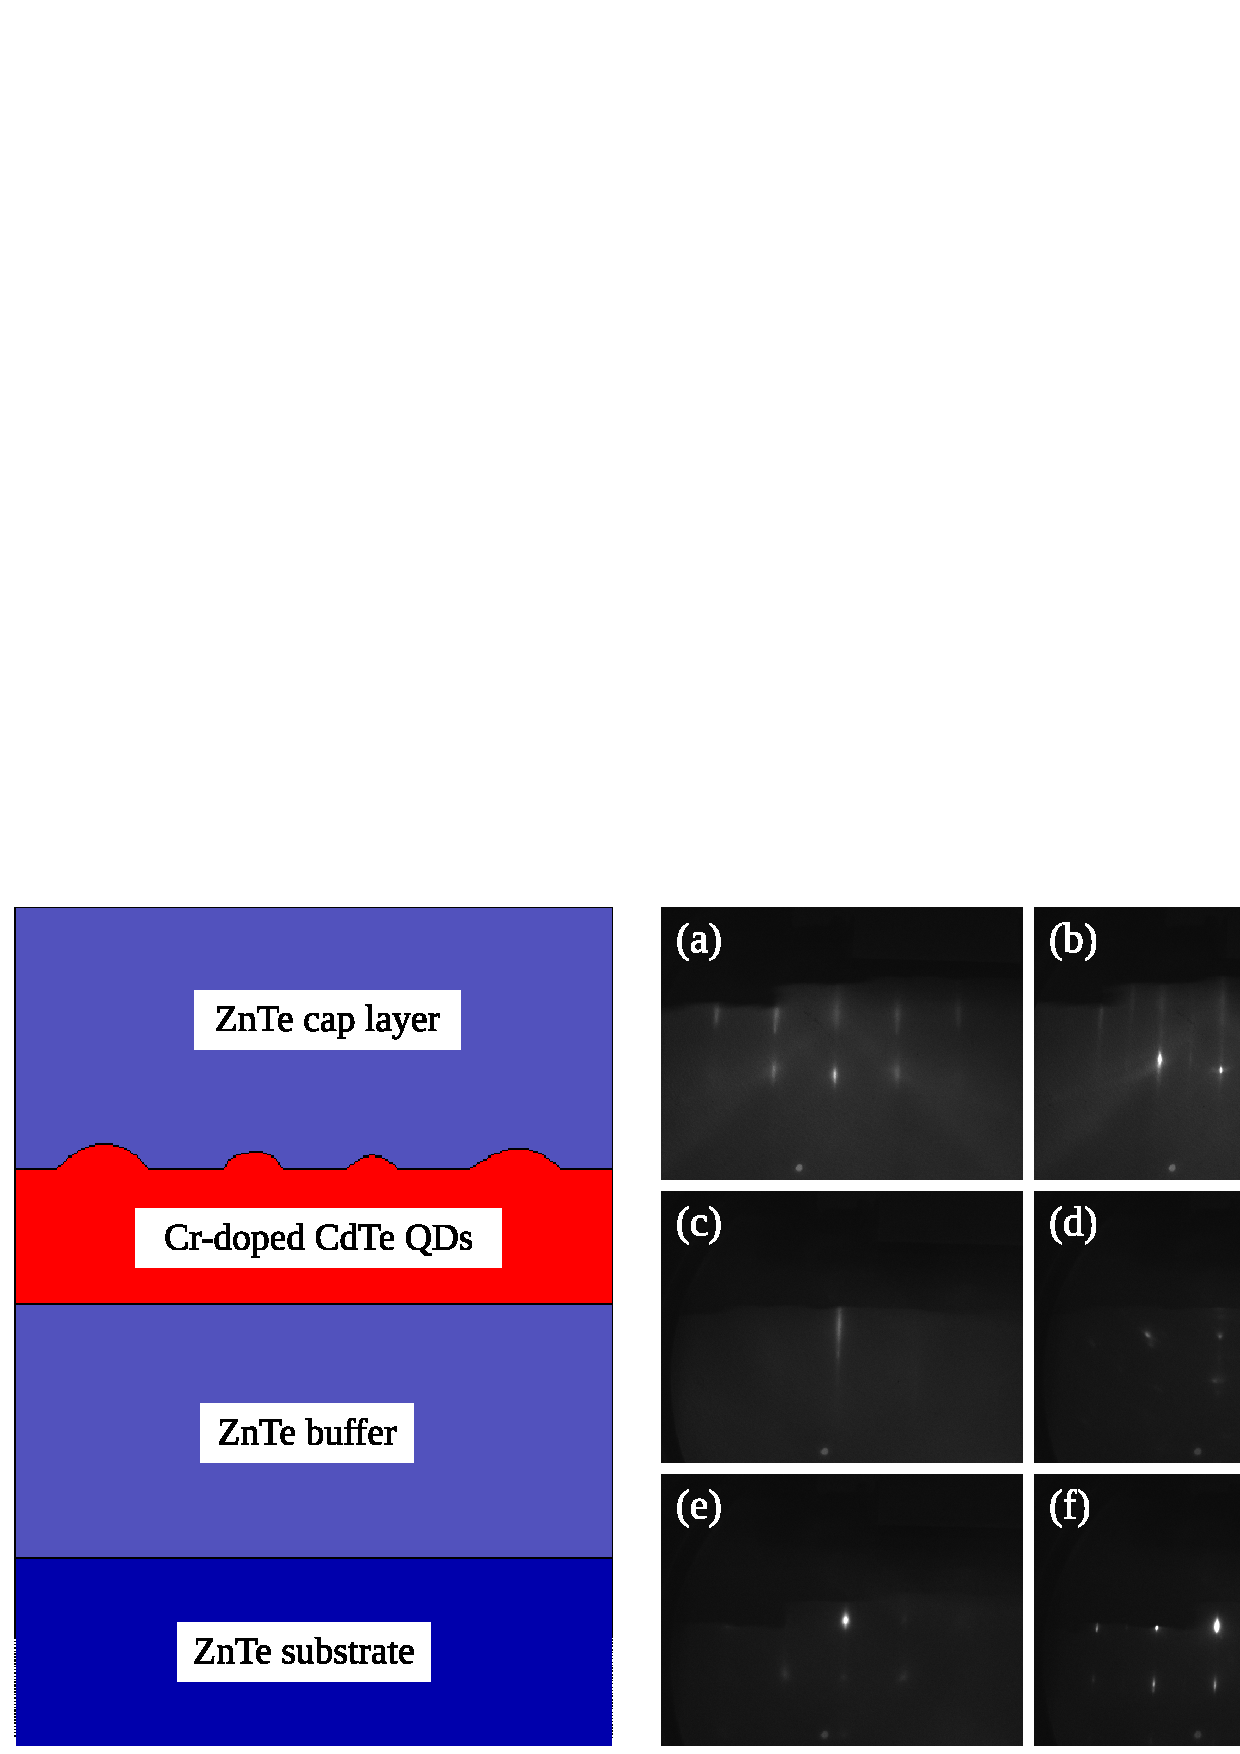
\includegraphics[width=14cm]{Pictures/RHEEDStep.png}
	\end{center}
	\caption{Left: Layer structure of the strain Cr-doped CdTe QDs samples. Right: RHEED pattern taken along the Te reconstruction line at different key moment of the growth: (a) before the growth of the ZnTe buffer, (b) after the growth of the ZnTe buffer, (c) end of the (Cd,Cr)Te layer deposition, (d) after the Te deposition, (e) after the Te evaporation (T$_{substrate} = 163^{\circ}$C) and (f) after the growth of the ZnTe cap.}
	\label{RHEEDStep}
	\end{figure}
	
	We begin the growth by opening the Zn cell shutter at a substrate temperature of $355^{\circ}$C. The substrate temperature was then raised to $400^{\circ}$C in a Zn atmosphere in order to flatten the surface for the growth. While it took several minutes to raise the substrate temperature, the growth was stopped by the auto-regulation of the ZnTe growth. When the substrate temperature reaches $400^{\circ}$C, the Te shutter was also opened, in order to grow the ZnTe buffer layer. This thick ZnTe layer keeps the dots far from the substrate surface, that can have some defects, and gives us a flat surface~\cite{ChangZnTe}. The surface quality is checked by RHEED, presenting clear diffraction lines (Fig.~\ref{RHEEDStep} (b)). The substrate temperature was then lowered to $295^{\circ}$C, the Zn cell being open until the temperature reach $355^{\circ}$C.
	
	CdTe is grown by ALE, in which the choice of substrate temperature fixes the quantity of material deposited at each cycle. It was found that 0.5 ML of CdTe is deposited at each cycle for a substrate temperature between 260$^{\circ}$C and 290$^{\circ}$C~\cite{HMarALE}. Taking a temperature between those two limits allows for a small uncertainty on the substrate temperature while keeping a really good control on the growth of the sample.
	
	The growth during ALE was monitored via the intensity of the specular spot. Focusing on the lowest angle reflected spot, called the specular spot, one can see small variations in the reflected intensity during the growth. This is the same mechanism as the one presented in Fig.~\ref{RHEED} for the RHEED oscillation during the construction of the surface. Fig.~\ref{RHEEDOsc} presents oscillations taken during an ALE. Low intensity moments correspond to Cd deposition, high intensity to Te deposition. One can see that the intensity varies in sequence of low intensity, high intensity, medium intensity and high intensity. Those corresponds to two ALE cycles, and therefore the growth of single CdTe monolayer~\cite{HMarALE}. We can also see the relaxation of a layer: the surface becomes then rougher, and the specular sport stays at low intensity.
	
	\begin{figure}[h!]
	\begin{center}
		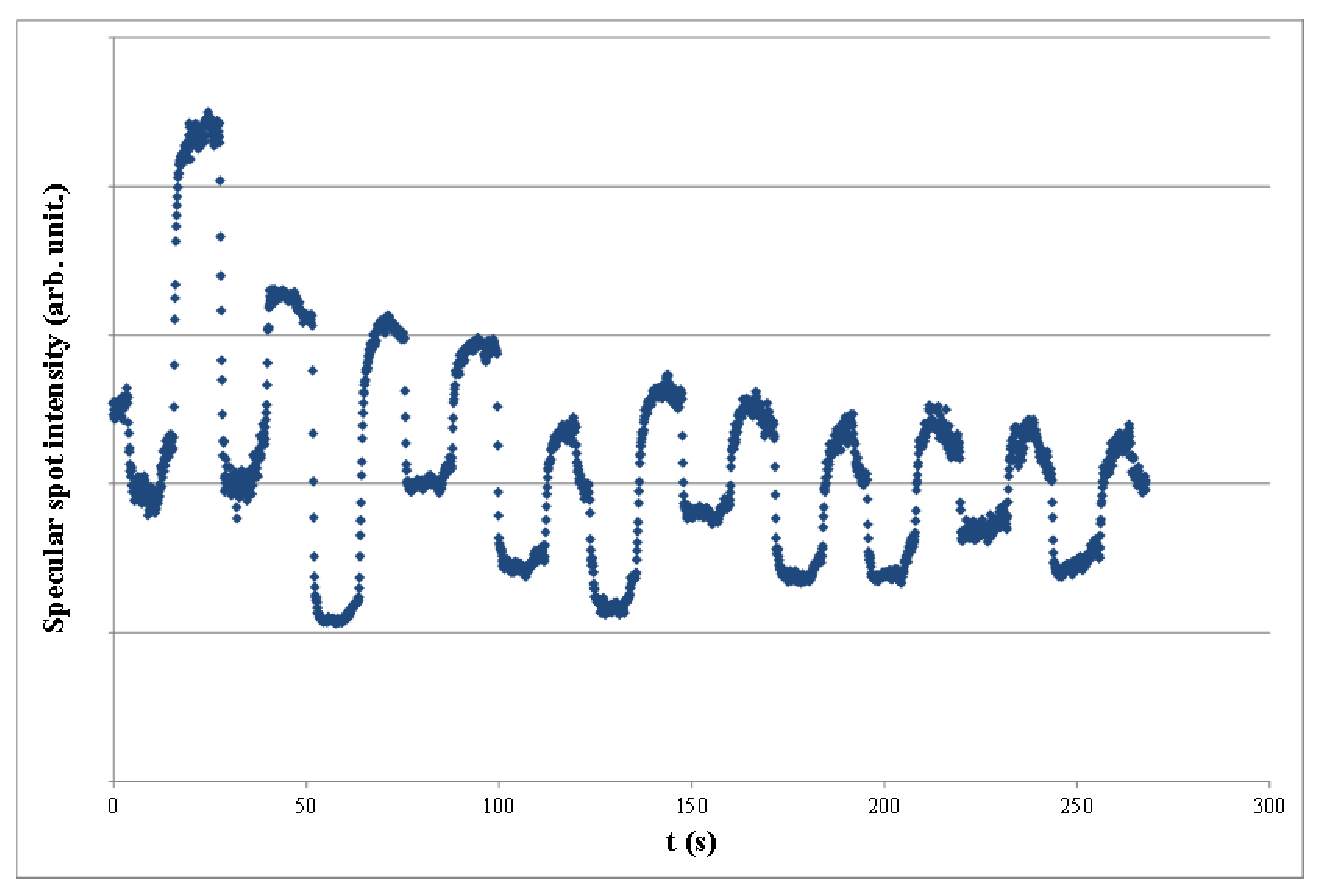
\includegraphics[width=12cm]{Pictures/RheedOsc.eps}
	\end{center}
	\caption{RHEED oscillation for the ALE of the strained dots.}
	\label{RHEEDOsc}
	\end{figure}
	
	One of the main goal of this work was to calibrate the Cr flux in order to optimize the probability of having a single Cr atom in most of the QDs of the sample. A first guess is that the Cr density must be of the same order as the QDs density at the surface of the sample. Supposing that all the Cr atoms get adsorbed on the sample, the quantity of deposited atoms is given by the flux of Cr times the time during which the cell stays open (exposure time). Due to the opening and closing time of the shutter, the exposure time cannot be shorter than a few seconds. Therefore a really small flux has to be chosen, with a BEP of the magnitude of $10^{-9}$ Pa, which is of the same order of magnitude than the main chamber pressure. It cannot therefore be reliably measured using the gauge pressure. In order to find the cell temperature needed to reach such a small flux, we used Arrhenius law, stating that the log of the flux of a cell varies linearly with the inverse of its temperature. From flux measured at higher temperature, we calculated the coefficients and deduced the aimed temperature of the Cr cell. The resulting curve is presented on Fig.~\ref{ArrLaw}, with the fit. The optimisation was done starting with the know how acquired in Grenoble on the growth of CdTe/ZnTe QD doped with single Mn and trying to optimise it for the Tsukuba machine, through a feedback with the micro-PL characterization in Grenoble.
	
	\begin{figure}[h!]
	\begin{center}
		\includegraphics[width=12cm]{Pictures/ArrheniusCr.png}
	\end{center}
	\caption{Cr BEP as a function of 1000/T. Parameters of the Arrhenius law are given in the top right.}
	\label{ArrLaw}
	\end{figure}

	This really small flux was achieved by heating the Cr cell around 1000$^{\circ}$C, and opening the cell only once during the deposition of the CdTe layer. In order to have QD emitting in the right range of wavelength for our optical setup (around $\lambda = 600$ nm), the optical CdTe thickness is 6.5 MLs. However, this is close to the critical thickness. Therefore, to diminish the risk of dislocation in the CdTe layer, some samples were grown with 5.5 MLs of CdTe. The Cr cell was opened when half of the CdTe layer was grown (7th cycle for the 6.5 MLs samples, 5th cycle for the 5.5 MLs samples). The ALE sequences used to grow the CdTe layer is shown in Fig.~\ref{RecipeSK}.
	
	\begin{figure}[h!]
	\begin{center}
		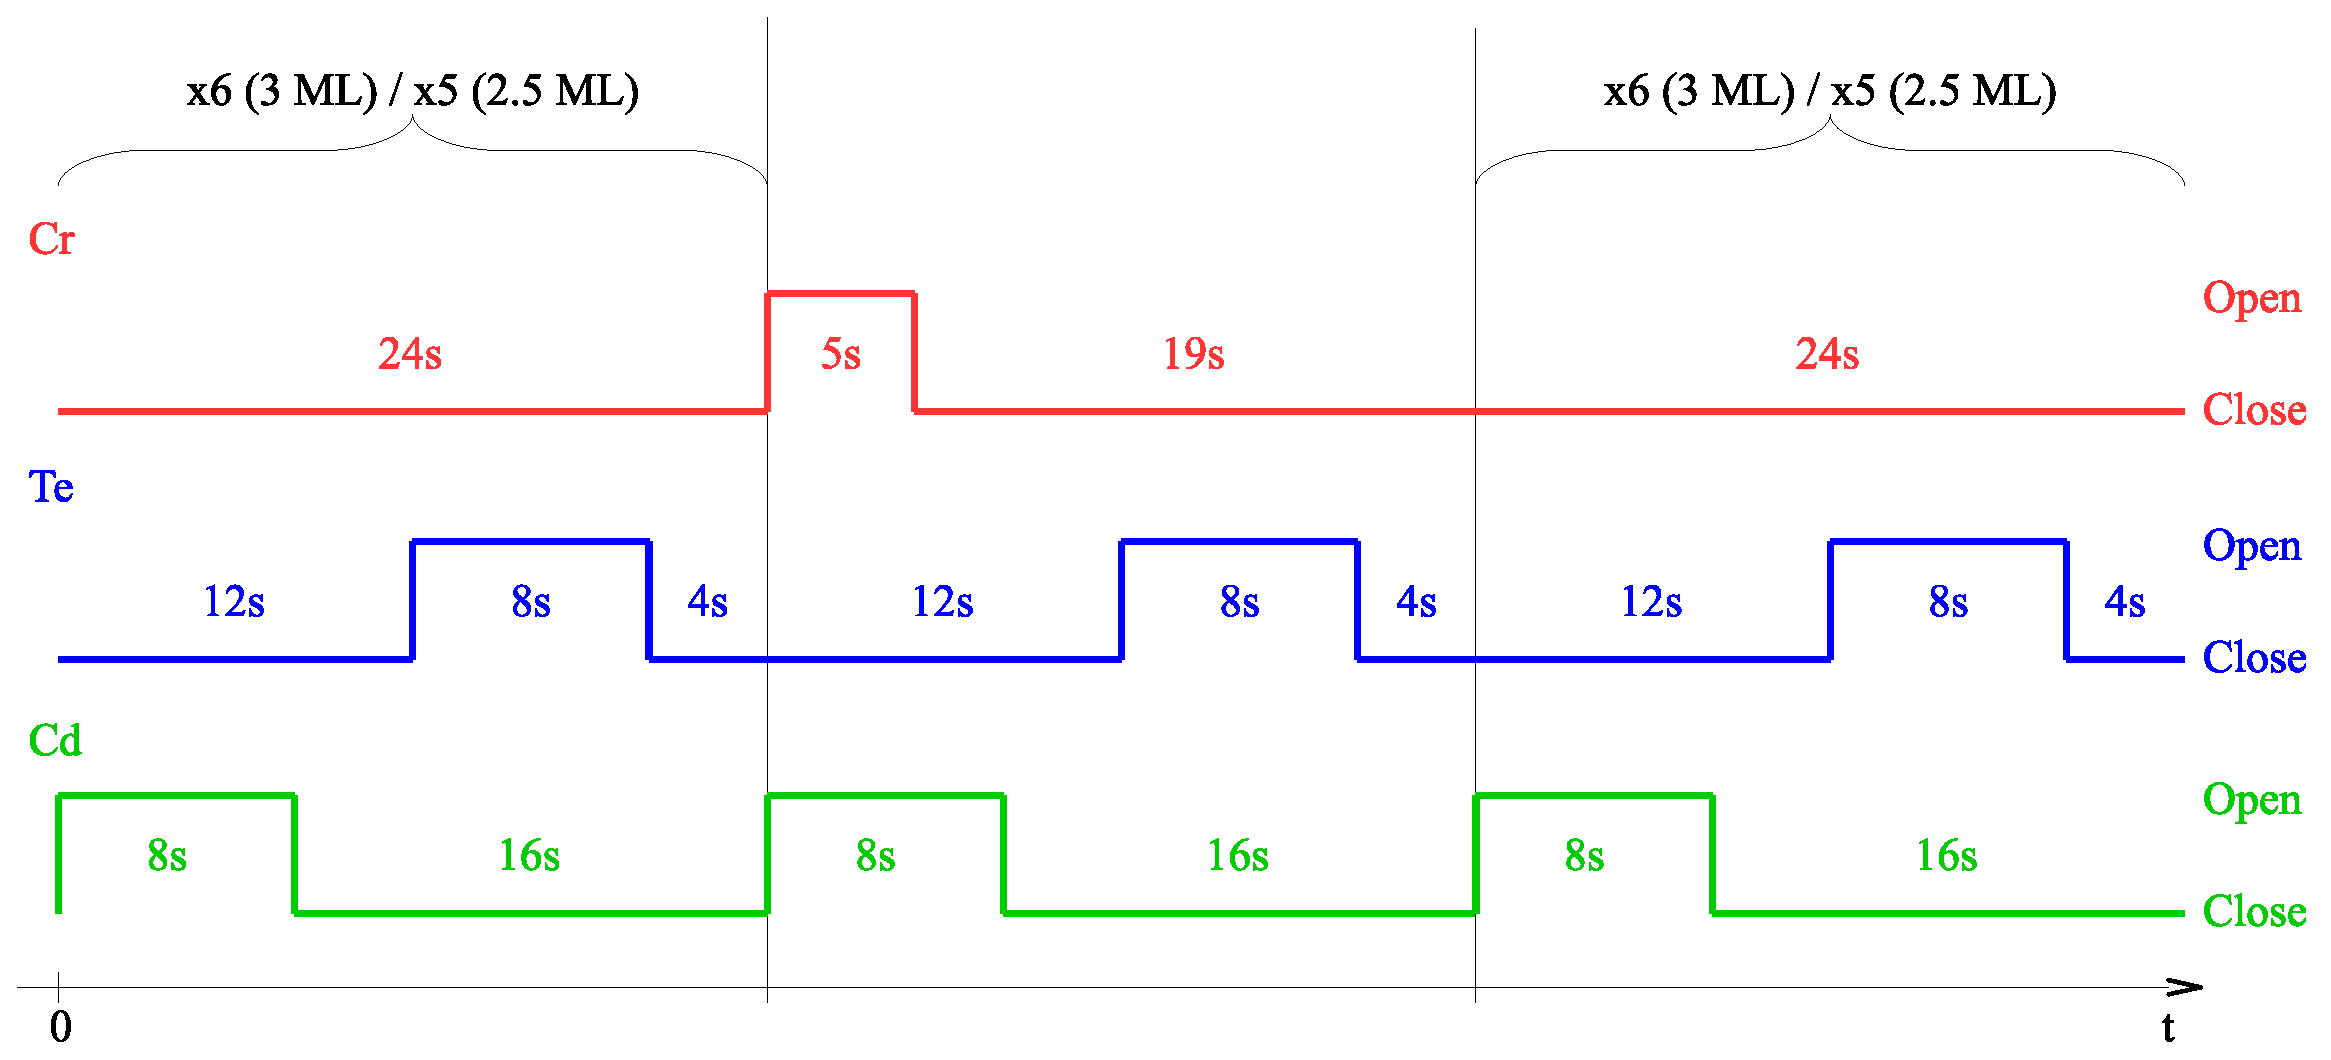
\includegraphics[width=13cm]{Pictures/RecipeSK.eps}
	\end{center}
	\caption{Opening and closing cycles of each cells used to grow either 6.5 MLs or 5.5 MLs of (Cd,Cr)Te for the formation of Cr-doped SK dots.}
	\label{RecipeSK}
	\end{figure}

	After the growth of the CdTe layer, we lowered the substrate temperature to $210^{\circ}$C to deposit an amorphous Te layer. It was deposited during 5 minutes. We then heated up the substrate again to $320^{\circ}$C, where we stayed for 20s in order to evaporate all the deposited Te~\cite{WojnarMBE}. The formation of dots was confirmed by a spotty diffraction pattern like the one presented on Fig.~\ref{RHEEDStep} (f). The Zn and Te cells were then opened, while the substrate temperature was raised to $350^{\circ}$C in order to grow a protective layer of about 50 nm of ZnTe above the QDs.
	
	\subsection{Optical characterization}
	
	The samples were studied in Grenoble, at the Neel Institute. The characterization of the samples was done in two steps. First, we took macro-photoluminescence spectra, on a large energy range, typically between 1.8 and 2.3 eV, with a laser set at 2.9 eV. This allow us to test the PL of the sample. As described in Sec.~I.3.2%~\ref{CrSemiCon}
, if the Cr concentration is too high, it may kill the PL of the dot layer, and thus it will not be seen in the macro-PL.
	
	If luminescence from the sample is seen in macro-PL, the sample is studied by micro-photoluminescence ($\mu$-PL), on a much narrower energy band (about 10 meV), to study dots individually. A high refractive index ($n \approx 2.5$) hemi-spherical Solid Immersion Lens (SIL) was mounted on the sample before their study, to improve the spatial resolution and enhance the collection efficiency of a single dot photoluminescence (PL) in a low temperature optical microscope. The sample is scanned randomly. We judge the quality of the sample by the number of actual dots we found with single Cr embedded inside, and by the proportion of sharp emission peaks (a few tens of $\mu$eV) versus broad ones (in the meV range): if we saw mainly broad peaks, it suggests that the Cr concentration is too high.
	
	\begin{table}[h!]
		\begin{center}
			\caption{List of samples where single dots with single Cr was found.\label{SKsamples}}
			\begin{tabular}{M{2cm}|M{3cm}|M{2cm}|M{3.3cm}|M{2.2cm}}
				Sample name & Cleaning process & \# CdTe MLs & Targeted Cr concentration (\%) & \# Cr-doped dots found\\
				\hline
				dot334 & Br etching & 6.5 & 0.09 & 3 \\
				dot338 & Br etching & 6.5 & 0.05 & 2 \\				
				dot359 & Br etching & 6.5 & 0.11 & 1 \\
				dot363 & Br etching & 6.5 & 0.21 & 2
			\end{tabular}
		\end{center}
	\end{table}
	
	The samples where QDs doped with a single Cr atom were found are listed in Tab.~\ref{SKsamples}. The Cr concentration in the sample was estimated using the Cr flux. The Cr composition is given as percentage of the cation site occupancy (Cd$_{1-x}$Cr$_x$Te). We see that optimal samples were found for a large range of concentration. The probability to find good Cr-doped dots in dot338 and dot363 is about the same. However, dot363, with the higher Cr targeted concentration, presents a lot of broad peaks. All samples grown with a Cr concentration higher than 0.20\% had a luminescence too weak to be studied properly. We can estimate that the good range of concentration is between 0.05\% and 0.20\%. Some more test have to be done in order to fine tune the Cr composition.
	
	\section{Charge tunable samples and strain-free samples}
		\subsection{Charge tunable samples\label{ChargedSample}}	
		
	Samples with contact on the back and on the surface were grown in order to control the charge ofthe studied QD via the application of an electric field. The growth was done on a p-doped ZnTe substrate to have a conductive back contact on the sample. The growth of the SK dots was done with the procedure described in the previous section. The substrate of the charge tunable samples were cleaned using H$^*$ plasma. Thinner buffer and cap layers was necessary in order to be able to apply a stronger electric field on the dot layer. We chose thicknesses between 150 nm and 200 nm for the buffer, and of 110 nm for the cap.
	
	\begin{figure}[h!]
	\fcapside{\caption{Schema of the charge control structure, on a p-doped ZnTe substrate and with a thin, semi-transparent gold layer deposited on the surface.}\label{ChargeContSample}}	
	{\begin{center}
		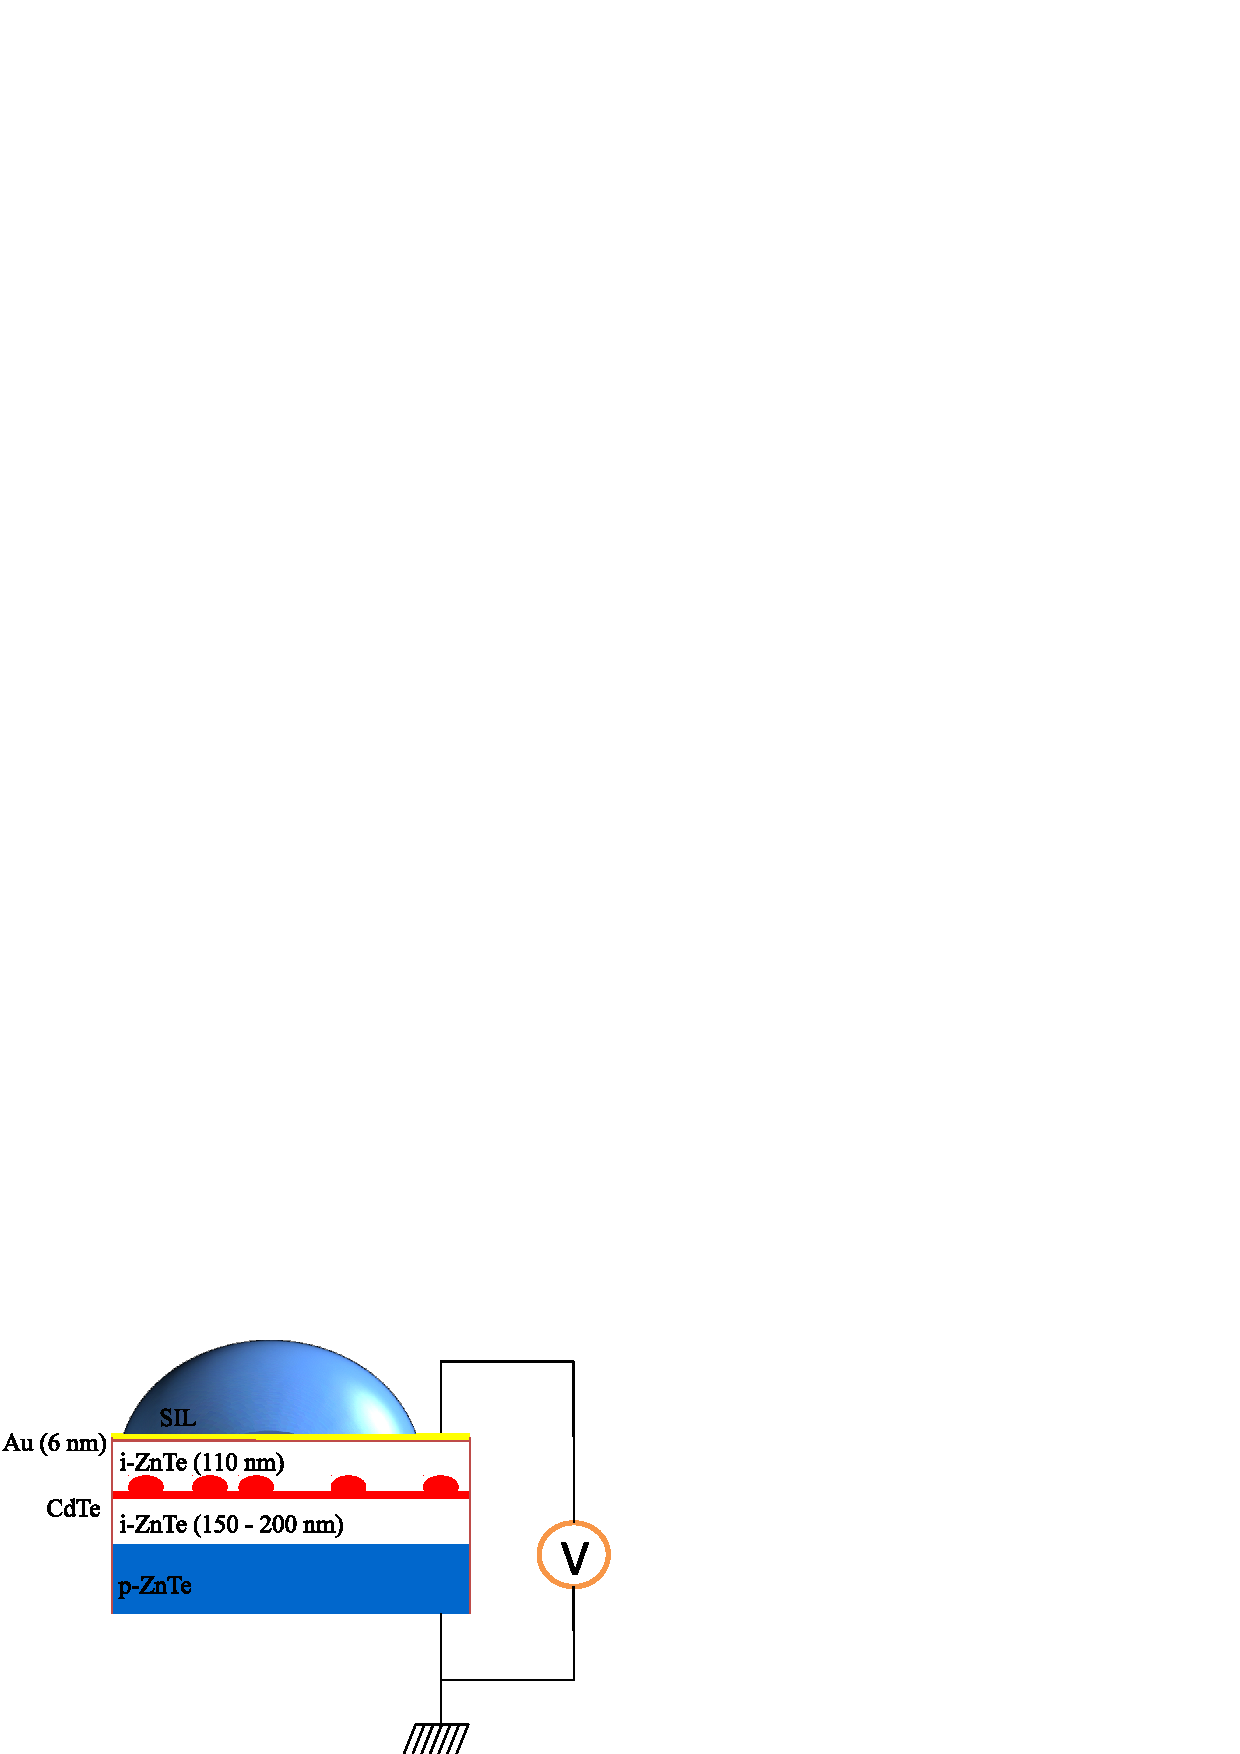
\includegraphics[width=7.4cm]{Pictures/ChargeContSample.png}
	\end{center}}
	\end{figure}
	
	The conductive surface contact was formed by a thin, semi-transparent gold layer, forming a Schottky junction with the sample cap layer. It was deposited by sputtering just after the MBE growth in order to keep a clean surface. The samples were kept in nitrogen atmosphere during the transport between the MBE and the sputtering machine. A deposition time of 35 s was chosen. Fig.~\ref{ChargeContSample} shows a schema of the sample as it was studied.
	
	Only one Cr-doped charge tunable sample was grown and studied during this PhD, named dot390. It was decided to make the CdTe layer 5.5 MLs thick in order to have no dislocation in the QD layer. The targeted Cr concentration was 0.16\%.
	
 	\subsubsection*{Optical characterization}
	
	In order to test the application of bias voltage in the sample, we glued two electrodes with silver lacquer. A SIL was mounted on top of the sample. We looked at the PL of single dots and see their evolution under the application of a bias voltage. Fig.~\ref{ChargeVar} (a) presents the results of such an experiment for a dot with no Cr embedded.
%	 One can notice that all the emission energy of all the species change under application of an electric field.

	\begin{figure}[h!]
	\begin{center}
		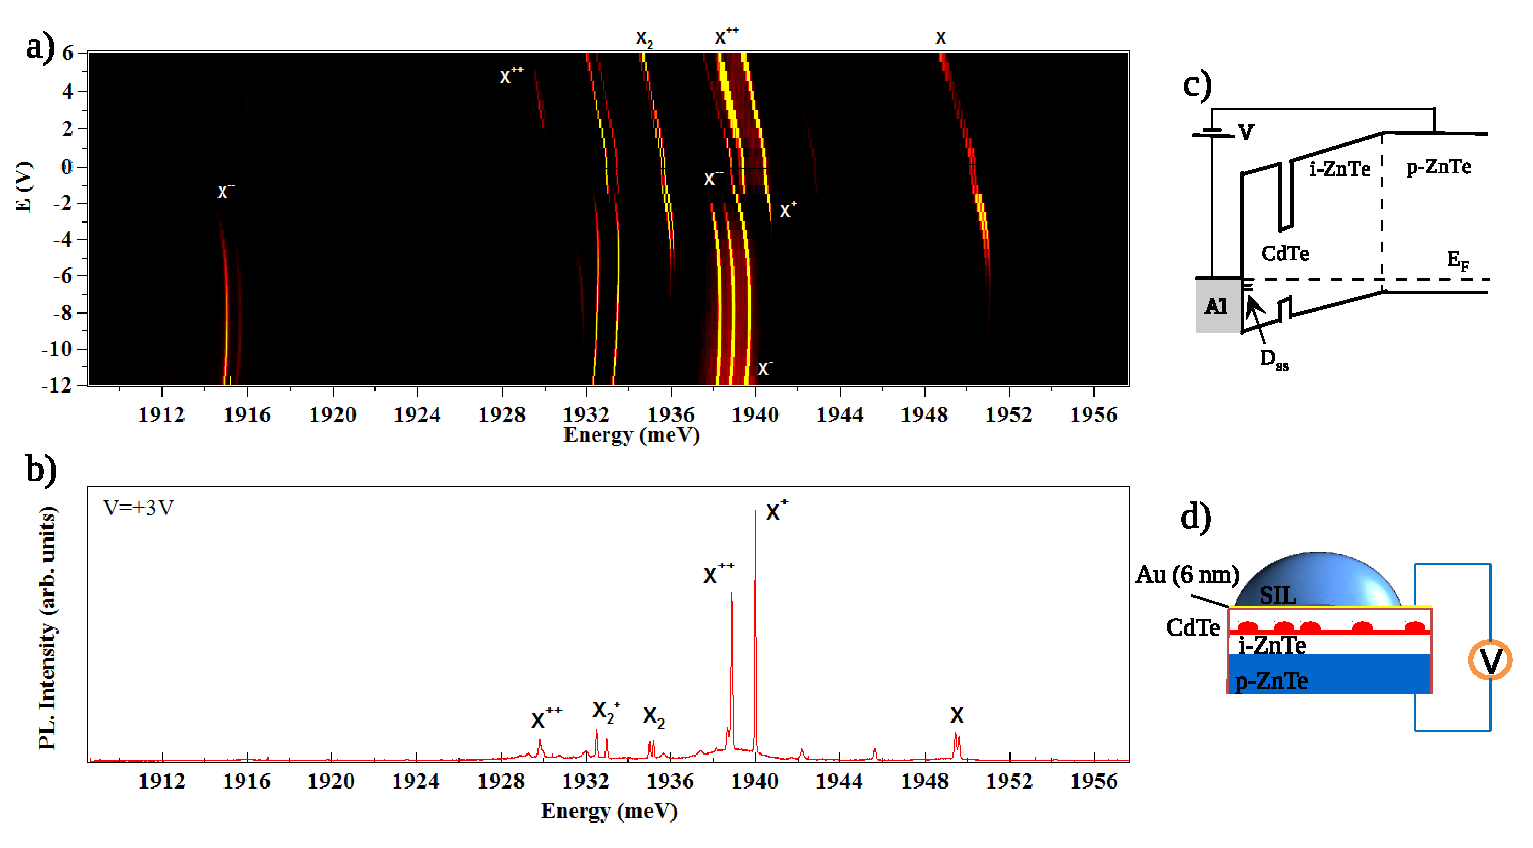
\includegraphics[width=12cm]{Pictures/MapEfield.eps}
	\end{center}
	\caption{(a) Evolution of the PL of a single dot under application of a bias voltage V. Below are presented spectra of the dot taken under three different values of bias voltages: (b) V = $+3$ V (positively charged), (c) V = $-1.5$ V (neutral) and (d) V = $-8$ V (negatively charged). Identification of the different species was done following ref.~\cite{BesombesIdentificXSpecies}.}
	\label{ChargeVar}
	\end{figure}

	The main result of the experiment is the appearance of different excitonic species depending on the applied electric field. The spectrum are dominated by the neutral state of the quantum dot for an applied electric field of V = -1.5 V (Fig.~\ref{ChargeVar} (c)). At this voltage, the neutral excitonic species X and X$^2$ are the strongest. Charged excitons still appear because of charge variations occuring close to the QD, injecting electron or holes inside it. Further lowering the bias voltage, the probability of the dot to be negatively charged increases. Neutral excitonic species disappear and the peaks of the negatively charged species (X$^-$, X$^{--}$ and X$_2^-$) become dominant. A spectra taken at V = -8 V is presented on Fig.~\ref{ChargeVar} (d). One can notice that, X$^{--}$ is splitted into two group of two peaks, around 1917.5 meV and 1933 meV on Fig.~\ref{ChargeVar} (d). This structure is dominated by the electron-electron exchange interaction and has already been observed in InAs QDs~\cite{FineStructX2charge}. On the contrary, applying a positive bias voltage increases the probability to detect positively charged exciton complexes, maximizing X$^+$ and X$^{++}$ intensity. This is shown on Fig.~\ref{ChargeVar} (b) for a bias voltage of V = +3 V. A structure of two doublet is also observed for X$^{++}$. This shows that we can select efficiently the charge of a quantum dot applying a bias voltage across the sample.
%	We see for example that, for a bias voltage of +3 V (Fig.~\ref{ChargeVar} (b)), the neutral species are almost extinguish and the charged species X$^+$, X$^{++}$ and X$_2^+$ have the more intense PL. Similarly, at negative electric field, only the charged species X$^-$, X$^{--}$ and X$_2^-$ remain, X$^{--}$ and X$_2^-$ disappearing for an applied bias voltage higher than -2 V. This shows that we can select efficiently the charge of a studied quantum dot applying a bias voltage on it.
	
%		Fig.~\ref{ChargeVar} (c) gives a schematic view of the Schottky gate. In this compound, the Fermi levels of the metal, semiconductor and p-doped semiconductor align via Fermi level pinning. Applying a bias voltage to the back and front of the sample change the position of the Fermi level, and therefore the probability of injection of hole or an electron in the dot, depending on the direction of the applied voltage. Moreover, the energy barriers at the interfaces keep the current to flow in the non-doped part of the semiconductor. We can then apply an electric field on the sample, and thus control the charge of the sample, without having a current going through it.
	
	No Cr doped quantum dots were found in dot390. Some dots looking like dots doped with a single Cr atom were observed, but detailed investigation shows no sign of magnetic atom in them. The properties of such QDs are discussed in more details in Sec.~\ref{ChargeFluc}.
	
		\subsection{Strain-free quantum dots\label{SFD}}
		
%		The strain-free dots are formed by the interface variation of a thin (about $4ML$) CdTe quantum well (QW) between CdMgTe layers. These thickness variations will create dots, in which we will want to include a single magnetic atom. The whole structure is ideally grown on a CdTe substrate, in order to have absolutely no strain in the dots layer.
%		
%		However, there was no CdTe substrate in Tsukuba. So, we had to grow a thick layer of CdTe in top of GaAs substrate, which a lattice parameter close to CdTe, on order to have a completely relaxed surface to do our growth.
%		
%		To achieve so, we start by cleaning the GaAs substrate. It was done in four step outside the MBE chamber, all of them using an ultrasonic cleaning. It was first immersed in acetone, during 5 minutes, with the ultrasonic frequency at $43MHz$. Staying at this frequency, it was then immersed in ethanol during 5 minutes again, and then in water for the same time. We finished with a last 5 minutes cleaning in water, at $23MHz$ this time.
%		
%		Putting the substrate in a chamber, we proceeded to the last step of the cleaning: hydrogen radical (H$^*$) cleaning, created by injecting nitrogen radical in a chamber of H gas, in order to remove Ga oxyde formed at the surface while transporting the sample. We check the final composition of the gas via the electron energy using optical probing. For a H$^*$ gas, this should be round 660nm. To achieve the H radical cleaning, we heat the GaAs substrate to $400^{\circ}$C and then open the valve between the main chamber and the one containing H$^*$ gas. We exposed it for 15 minutes, and then searched for line in the RHEED pattern, to check the quality of the cleaning. during this step, and also during the growth, the sample was rotating.
%		
%		Once the cleaning process is finished, we began the growth of the thick layer of CdTe. We began by a very thin layer of ZnTe in order to relaxed some of the strain. Staying at T$_{substrate} = 400^{\circ}$C, we first opened the Zn cell for 30s, then opened both Zn and Te cells for 50s, before closing again Te cell. We then go down to T$_{substrate} = 250^{\circ}$C under Zn flux and, once the temperature was stabilized, closed the Zn cell and proceeded to the CdTe layer growth, during 1h. Finally, once this layer was grown, we protected it from oxidation by adding a thin layer of Te while the substrate temperature was going down to $5^{\circ}$C.
%		
%		For this sample, only a simple cleaning occur outside of the MBE machine. We did it in four steps, each of them lasting for 5 minutes in an ultrasonic cleaning device. We began with a cleaning acetone, at 43 kHz, followed by one in ethanol at the same frequency. We then put the substrate in water and clean it at 43 kHz. Finally, we changed the water and did the last step in water at 23 kHz, in order to clean the substrate from smaller dust particle.
%		
%		Since the surface of the GaAs is oxidized, no RHEED pattern was visible, as shown on Fig \ref{Hybrid}(a). The desoxidation was done in the MBE main chamber, in vacuum condition, using hydrogen radical (H$^*$). In order to form the radical gas, a hydrogen gas was ionized in a chamber by a RF power source of 300 W and with a frequency of 13.6 MHz. This gas composition is optically checked by probing the emission of the Balmer serie: for a pure hydrogen gas, peaks at 656 nm and 486 nm appear clearly. During the formation of this gas, the substrate temperature is raised to $400^{\circ}$C. Once the hydrogen chamber is full of H$^*$ gas, we initiate the rotation of the sample. Since the chamber was situated just under the main and linked to her, we just had to open the shutter between the two to send the radical gas onto the substrate. We exposed the substrate to this gas for 15 minutes, under a pressure of about $6\times10^{-7}$ Torr. We then checked the sample surface with RHEED, which should present a streak pattern with some dots as presented in Fig \ref{Hybrid}(b). 
%		
%		Once the cleaning of the sample was finished, we closed the H$^*$ gas chamber shutter, waited for the ultra-high vacuum to re-established in the main chamber and began the growth of the CdTe layer. We grew it in two times: one hour of growth just after the cleaning (described here) and about four hours just before the actual growth of  the quantum dots structure.

%	The barrier for strain free samples are made of CdTe. The chosen substrate for the growth was GaAs, on which we grew a layer of about 3 $\mu$m of CdTe. Growing such a thick layer guaranty that the remaining strain are in the order of $0.1\%$ \cite{StrainRelaxCdTeGaAs111,StrainRelaxCdTeGaAs100}. Moreover, a small ZnTe layer was grown between GaAs and CdTe, which accelerated the relaxation of the strains \cite{StrainRelaxZnTeGaAs001}.
	
	In SK dots, large strains remain in the QD layer, and we have no control on them. As will be discussed later, remaining strains may prevent the observation of all the spin states of the Cr atom and limit the life-time of the Cr spin. We decided therefore to grow strain-free dot to get rid of those limits. They are formed by the thickness fluctuations of a CdTe quantum well in Cd$_{0.7}$Mg$_{0.3}$Te barriers, grown on a CdTe substrate. These fluctuations form steps localizing the carriers, acting as QDs. We chose to use Cd$_{0.7}$Mg$_{0.3}$Te to keep a lattice parameter close enough to CdTe to grow thick enough barriers, and keeping enough gap difference to localize the carriers. The needed flux for this growth are shown in Tab.~\ref{FluxTempSFD}.
	
	\begin{table}[h!]
	\begin{center}		
		\begin{tabular}{| c | c | M{4cm} |}
			\hline
			Elements & Targeted BEP (Pa) & Targeted flux (atoms.cm$^{-2}$.s$^{-1}$) \\ \hline
			Cd & $6.0\times10^{-5}$ & $6.7\times10^{13}$ \\
			Mg & $2.1\times10^{-6}$ & $4.7\times10^{12}$ \\
			Te & $7.0\times10^{-7}$ & $5.8\times10^{13}$ \\
			\hline
		\end{tabular}
		\caption{Aimed flux for each cell during the growth of the strained samples.}
		\label{FluxTempSFD}
	\end{center}
	\end{table}
	
	The critical thickness of Cd$_{0.7}$Mg$_{0.3}$Te on CdTe is not exactly known. Systematic studies were done on CdTe/CdZnTe gives an empirical law to calculate the critical thickness~\cite{CritThickCdTeCdZnTe}. This law was used for different II-VI material and gives a good approximation of the different critical thickness, overestimating slightly the effects of strain. For CdTe/Cd$_{0.7}$Mg$_{0.3}$Te, we found a critical thickness $h_c = 130$ nm. We chose to grow 40 nm below the quantum well (QW), and 90 nm above it, to keep the surface far from the quantum well.
	
	The strain-free sample were grown on a hybrid substrate formed by a thick CdTe layer grown on GaAs. It was done on a fourth of a 2 inches GaAs substrate and protected by Te. The GaAs substrate was cleaned using H$^*$ plasma. A thin layer (about 7 nm) of ZnTe was first grown at 415$^{\circ}$C in order to get the right crystal orientation when growing the CdTe layer. We then grew a CdTe layer of about 3 $\mu$m at 360$^{\circ}$C, to recover a good crystallinity of the CdTe layer~\cite{StrainRelaxCdTeGaAs111}. The RHEED taken after the growth of the CdTe layer (Fig.~\ref{Hybrid} (d)) shows sharp straight line, showing the recovery of a flat surface.

	\begin{figure}[h!]
	\begin{center}
		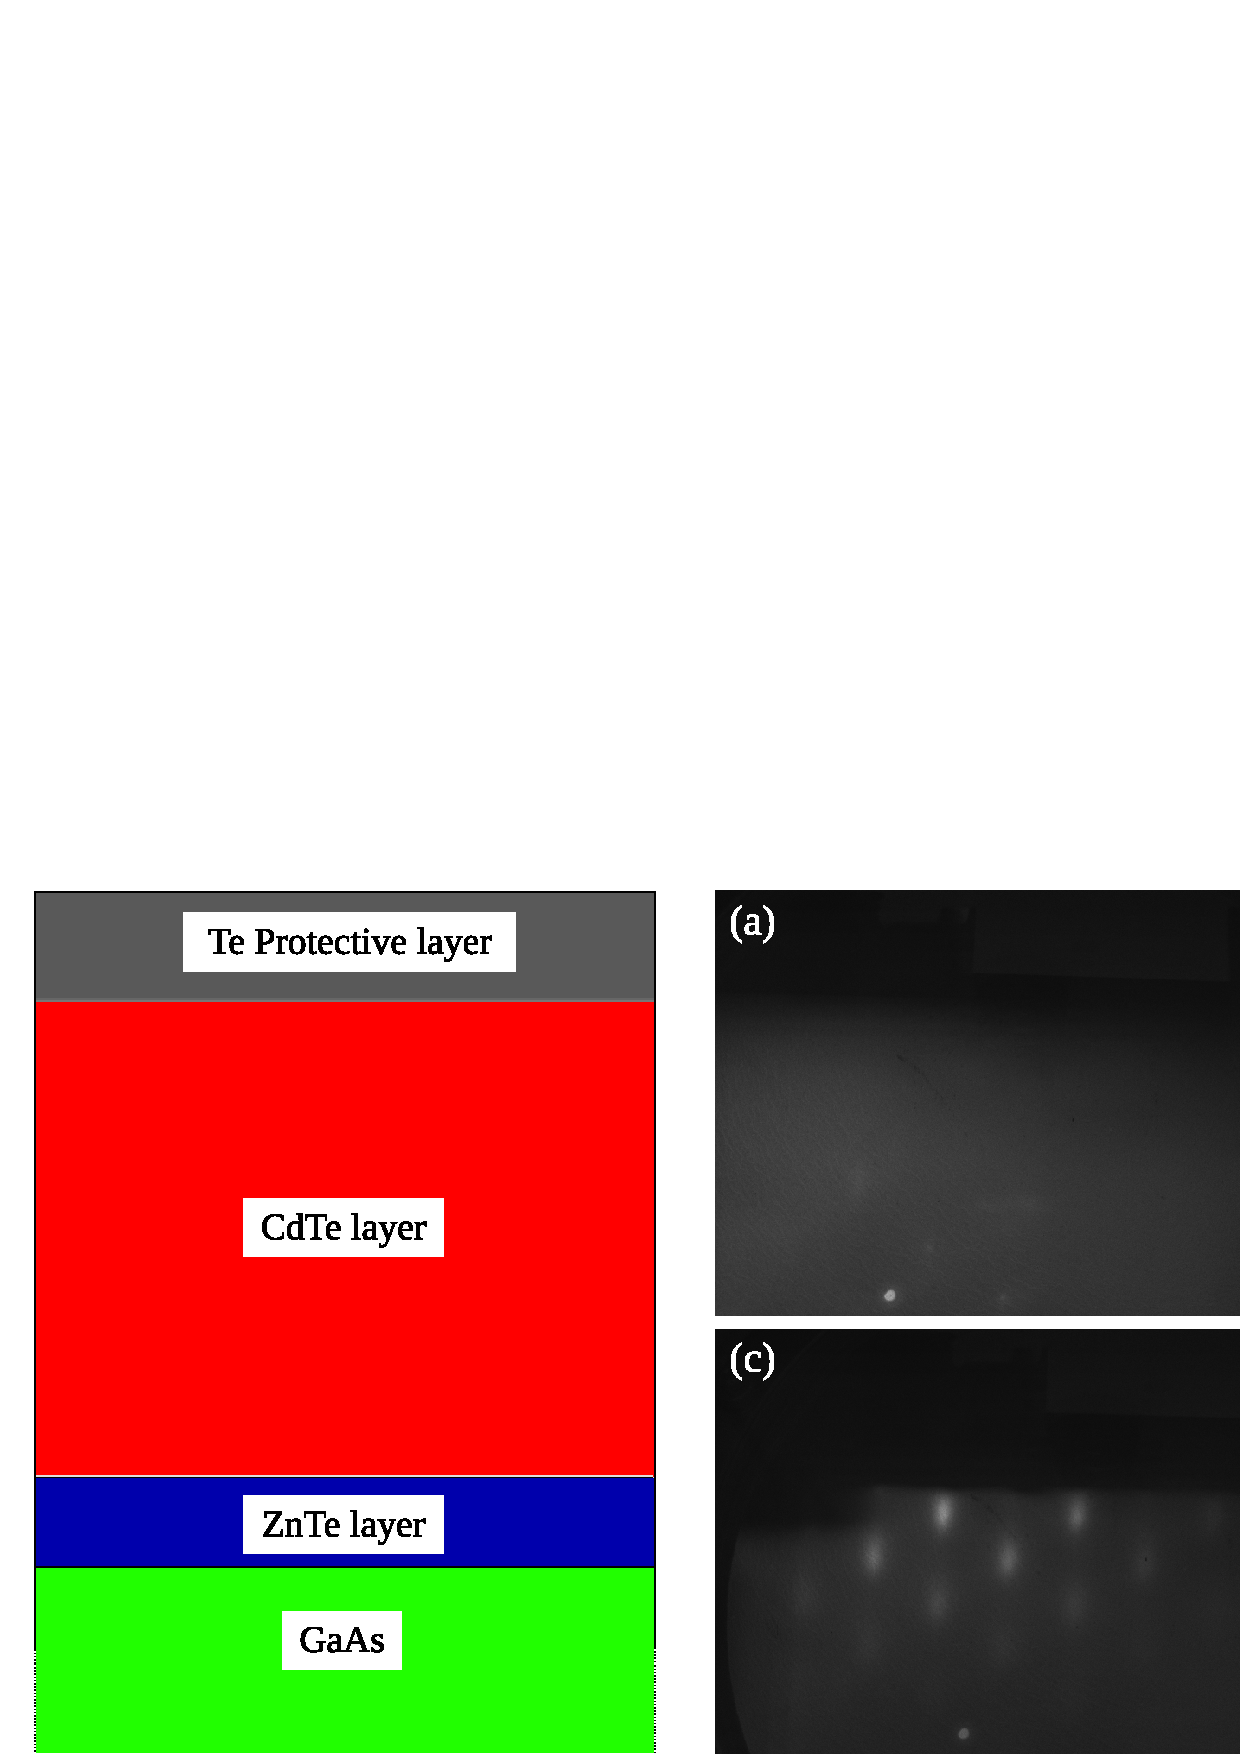
\includegraphics[width=14cm]{Pictures/HybridSubstrate.png}
	\end{center}
	\caption{Left: Layer structure of the hybrid substrate with its protective Te cap.
		Right: RHEED pattern taken at different key moment of the growth: (a) before H$^*$ cleaning of GaAs, (b) after H$^*$ cleaning of GaAs, (c) after the growth of the ZnTe layer, (d) after the growth of the CdTe layer.}
	\label{Hybrid}
	\end{figure}
		
%		This first part of the growth took place on a rotating sample. It only take about 15 ML of ZnTe on GaAs for the II-VI compound go back to its original lattice parameter \cite{StrainRelaxZnTeGaAs001}. Moreover, CdTe over ZnTe has a critical thickness of 5 ML \cite{CritThickCdTeZnTe}. So, to accelerate the relaxation of strain, we decided to grow a thing layer of ZnTe above the GaAs, before growing the CdTe thick layer. We lowered the substrate temperature to $320^{\circ}$C and opened the Zn cells for 30s with a BEP of $7.05\times10^{-7}$ Torr in order to flatten the surface. We then opened the Te cells, with a BEP of $5.21\times10^{-7}$ Torr, along with the Zn cell during 50s to grow the ZnTe layer in excess of Zn, making a layer about 7.2 nm thick.
%		
%		We then went to the growth of the first CdTe layer. We lowered again the substrate temperature to $250^{\circ}$C, under Zn flux. Once stabilized at the temperature, we closed Zn cells and open the Cd and Te cells for 1h. The Te cell had the same flux as previously, while the Cd cells had a flux of $4.72\times10^{-7}$ Torr. This layer was 633 nm thick, grown at 0.54 ML.s$^{-1}$. In order to protect the surface, we deposit an amorphous protective layer of Te above it, while decreasing the substrate temperature.
		
%	As said in the introduction, the strain free dots are formed by thickness variation of a CdTe QW surrounded by CdMgTe barrier. In order to have to good confinement while keeping a close enough lattice constant, we chose to use Cd$_{0.7}$Mg$_{0.3}$Te. Therefore, the first step of the growth was to chose the flux for the growth. We went through a process of trial and error, growing several samples and testing their composition with Electron Probe Mico-Analysis and X-Ray diffraction, as well as the thickness grown with a step gauge, in order to estimate the growth speed. Since we wanted to grow Cd$_{0.7}$Mg$_{0.3}$Te, we began the test with a ration Te:Cd of 1:0.7 and a ratio Te:Mg of 1:0.3. After five round of adjustment, we achieve the growth of Cd$_{0.7}$Mg$_{0.3}$Te, settling with the targeted flux presented in Tab.\ref{FluxTempSFD}.
%	For the settled Mg flux, the step gauge indicated a grown thickness of $520 \pm 5$ nm. Since we grew the test layer during 1h, we found a growing speed of about 0.15 nm.s$^{-1}$.
	
	For the growth of strain-free samples, we began to raise the substrate temperature to 300$^{\circ}$C and waited for a few seconds to remove all the deposited Te. We then heated the sample to $360^{\circ}$C. Starting at $320^{\circ}$C, we opened the Te cells in order to stabilize the surface. When the substrate temperature reached $360^{\circ}$C, we opened the Cd cells and grew a 2.35 $\mu$m of CdTe on top of the 3 $\mu$m grown on the hybrid substrate, in order to have a QW structure far from the surface that might have been slightly damaged during the conservation or the Te evaporation.
	
	\begin{figure}[h!]
	\begin{center}
		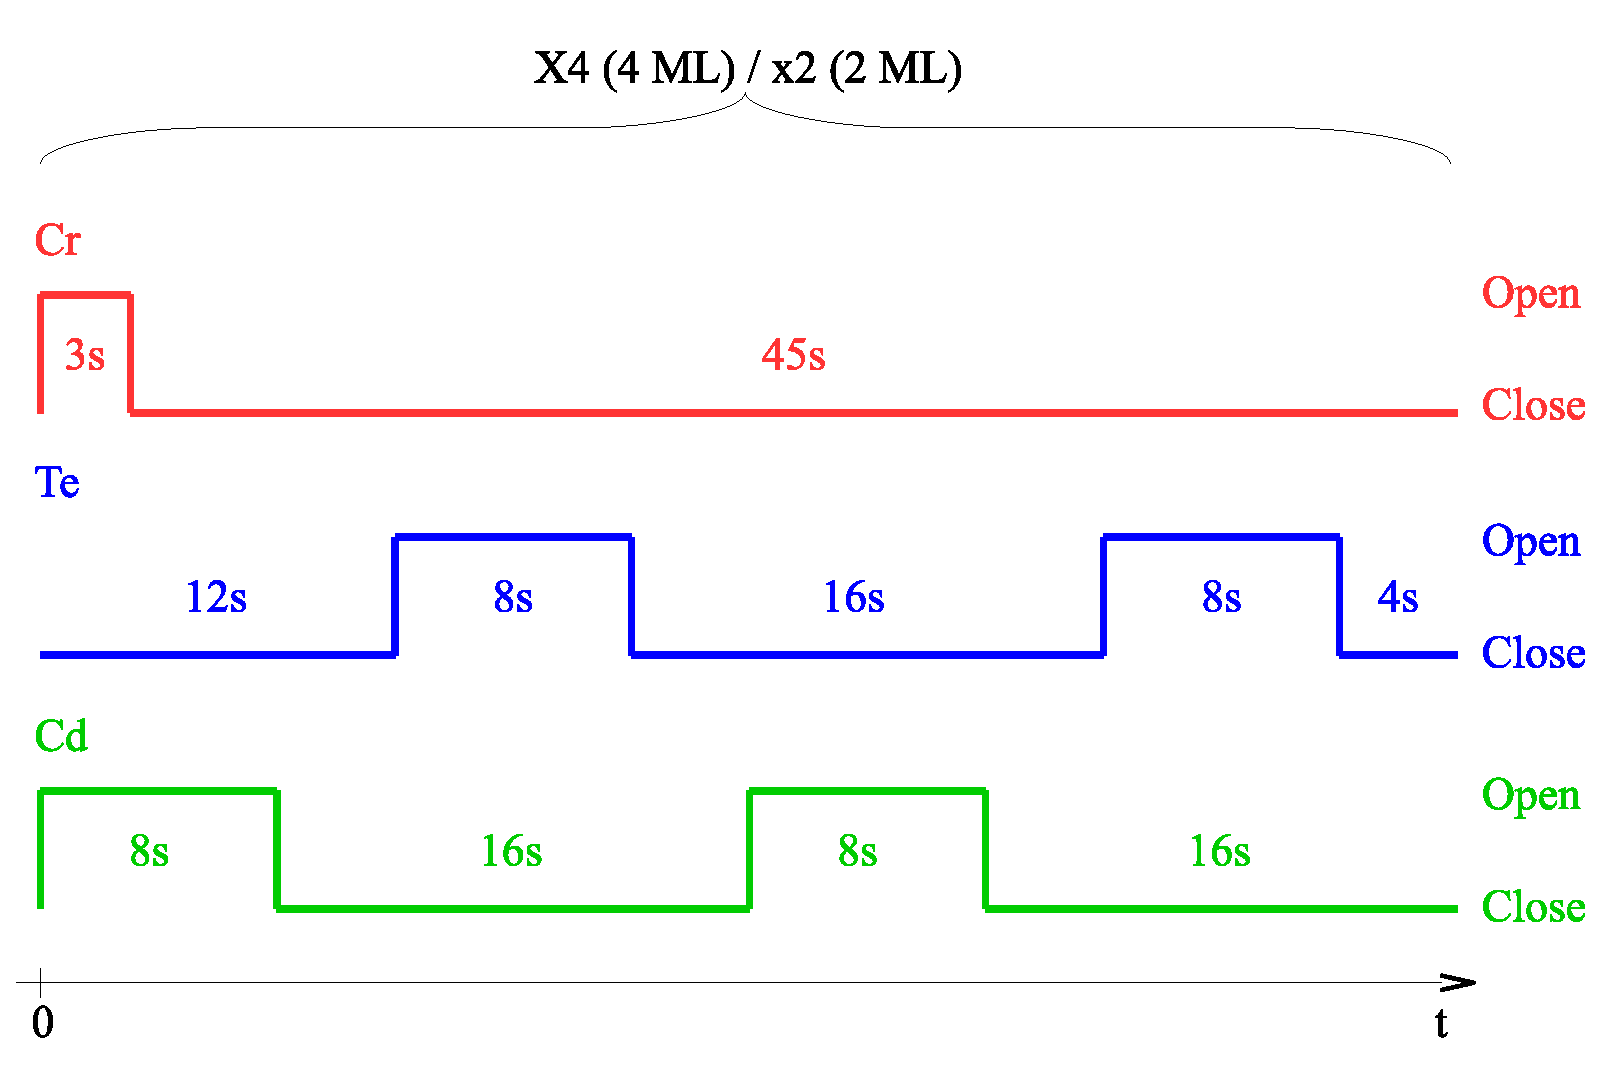
\includegraphics[width=10cm]{Pictures/RecipeSFD.eps}
	\end{center}
	\caption{Opening and closing cycles of each cell for the ALE of strain free (Cd,Cr)Te samples.}
	\label{RecipeSFD}
	\end{figure}
	
	We grew the 40 nm Cd$_{0.7}$Mg$_{0.3}$Te barrier on this buffer layer. Once the growth was done, we lowered the substrate temperature under Te flux, in order to smoothen the sample surface. Once the substrate temperature reached $295^{\circ}$C, we began the ALE of the QW. Two QW thicknesses were tested: 4 ML and 2 ML. The Cd and Te cycles were the same as for the SK dots. The Cr, however, was open for only 3 s, but once every two cycles, for a total of 4 opening in the 4 ML case, and 2 opening for the 2 ML case. The whole recipe is described in Fig.~\ref{RecipeSFD}.
	
	We then raised the substrate temperature up to $360^{\circ}$C, under a Te flux, in order to proceed to the growth of the upper barrier, acting also as a protective layer. The opening time was there calculated to grow 90 nm of Cd$_{0.7}$Mg$_{0.3}$Te.

	\subsubsection*{Optical characterization}
	
	Four samples of strain-free dots doped with Cr were produced (see Tab.~\ref{SFDsamples}). The Cr concentration were taken high because it was observed in the strain-free dots grown in Grenoble that a higher concentration of Mn was needed in strain-free dots than in SK dots. It was supposed to be the same with Cr. The Cr concentration was later raised after no dot doped with a single Cr was found.
	
	\begin{table}[h!]
		\begin{center}
			\caption{Strain-free QDs doped with Cr.\label{SFDsamples}}
			\begin{tabular}{M{2cm}|M{2.5cm}|M{3.5cm}|M{3cm}}
				Sample & \# CdTe MLs & Cr aimed concentration (\%) & Probability of Cr-doped QD \\
				\hline
				SFD4 & 4 & 0.35 & None found \\
				SFD5 & 2 & 0.15 & None found \\
				SFD6 & 2 & 0.54 & None found \\
				SFD7 & 2 & 0.35 & None found \\
				SFD8 & 2 & 0.75 & None found
			\end{tabular}
		\end{center}
	\end{table}
	
%	\begin{figure}[h!]
%	\begin{center}
%		\includegraphics[width=10cm]{../FillingPicture.png}
%	\end{center}
%	\caption{Example of dot fin in SFD}
%	\label{ChargeVar}
%	\end{figure}
	
	The sample presented sharp and intense peaks, as shown in Fig.~\ref{SpectraSFD}. It hints at a better confinement of the carriers in the QDs than the similar strain-free dots grown in Grenoble. This may be caused by higher steps than expected at the CdTe/Cd$_{0.7}$Mg$_{0.3}$Te interface.
	
	\begin{figure}[h!]
	\begin{center}
		\includegraphics[width=10cm]{Pictures/SFDSpectra.eps}
	\end{center}
	\caption{(a) Macro-PL of a SFD5. (b) Examples of spectra taken under $\mu$-PL in SFD5.}
	\label{SpectraSFD}
	\end{figure}
	
	As discussed in Sec.~\ref{XMn}, the presence of a magnetic atom splits the emission of the exciton into several peaks, the number depending on the spin of the magnetic atom. Such complex was not found in the strain-free samples. This may be caused by a problem in the Cr incorporation. The Cr is possibly not well embedded in the QW layer. More tests have to be done, depositing the Cr at different moment of the growth.
	
	Another possible cause of this absence could lie in the absence of strain. In SK dots, the presence of in-plane biaxial strains increases the probability of the Jahn-Teller deformation to occur along the $z$ axis. In strain-free dots, all direction are equivalent, and we expect two third of the Cr-doped dots to be undetectable because they are quantized in the plane, creating no splitting visible in our setup.
	
	In order to increase the probability for the Cr to be quantized along the $z$ axis, it is proposed to slightly strain the quantum well. This might be done by growing the sample on Cd$_{0.96}$Zn$_{0.04}$Te instead of CdTe. The lattice parameter of CdTe and Cd$_{0.96}$Zn$_{0.04}$Te have a lattice mismatch of only 0.3\%, so the strain created in the lattice should remain weak. They should however be enough to increase the probability of a deformation along the $z$ axis, making more dots visible in our experiments.
	
	\section*{Conclusion}
	
	We saw in this chapter how we grew the samples studied in the next chapters. The samples were characterized in Grenoble. SK dots with single Cr atom embedded were found and studied. New Cr concentrations were tested in Tsukuba after the feedbacks from Grenoble. More tests have to be done to increase the probability of finding dots doped with a single Cr atom.
	
	First steps toward new kind of samples were also done: strain-free QD with single Cr, and SK dots with single Cr embedded in a field effect structure. Localized carrier emission was detected in the former, and we successfully applied bias voltage on the later. However, for both, no Cr-doped dots were found. More tests have to be done to optimize their growth.
%
% 	We used the characterization of the samples done in Tsukuba to narrow down on a Cr flux for the growth of Cr-doped QDs, and we decided to aim for a Cr estimated concentration in the sample of  0.17\%. We then went to two other kind of sample: one enabling the application of an electric field on the dots, and one with strain free dots. The charge control samples growth was a partial success: we were able to apply an electric field on the sample, but no dot containing a single Cr was found. Strain-free dot presented promising fine peaks in their emission, but we were not able to find Cr in them either. More experiments will be done in order to successfully grow sample with the possibility of charge control, and strain-free dots.
%
%	In the next chapters, we will study the optical properties and the spin dynamics in the magnetic QDs grown in Grenoble (Chap.~\ref{CoDynMn}) and Tsukuba (Chap.~\ref{MagOptStud} and \ref{CrDyn}).

\printbibliography

\end{document}